\documentclass[11pt,a4paper]{book}
\usepackage[spanish,es-nodecimaldot]{babel}	% Utilizar español
\usepackage[utf8]{inputenc}					% Caracteres UTF-8
\usepackage{multirow}                       % Multifila en tablas
\usepackage{lscape}
\usepackage{graphicx}						% Imagenes
\usepackage[hidelinks]{hyperref}			% Poner enlaces sin marcarlos en rojo
\usepackage{fancyhdr}						% Modificar encabezados y pies de pagina
\usepackage{float}							% Insertar figuras
\usepackage[textwidth=390pt]{geometry}		% Anchura de la pagina
\usepackage[nottoc]{tocbibind}				% Referencias (no incluir num pagina indice en Indice)
\usepackage{enumitem}						% Permitir enumerate con distintos simbolos
\usepackage[T1]{fontenc}					% Usar textsc en sections
\usepackage{amsmath}						% Símbolos matemáticos
\usepackage{amssymb}
\usepackage{emptypage}                      % Dejar sin estilo las paginas vacias
\usepackage[Sonny]{fncychap}                % Capitulos con encabezado chulo :D
\usepackage{subcaption}

\usepackage{tikz}
\usetikzlibrary{positioning, arrows, shapes, automata}

% Ajustar tikzet
\tikzset{Node style/.style={thick, draw=black, circle, align=center, minimum width=70pt}}
\tikzset{
	->, % Hace que los arcos sean dirigidos
	>=stealth, % Hace que la punta de las flechas sean gruesas
	node distance=7cm, % Distancia minima entre nodos
}

\usepackage[
    backend=biber,
    style=numeric,
    sorting=ynt
]{biblatex}                                 % Gestion de bibliografia
\addbibresource{bibliography.bib}           % Archivo que contiene la bibliografia

\usepackage{xcolor}
\definecolor{backcolour}{rgb}{0.95,0.95,0.92}
\usepackage{listings}

\newcommand\YAMLcolonstyle{\color{red}\mdseries}
\newcommand\YAMLkeystyle{\color{black}\bfseries}
\newcommand\YAMLvaluestyle{\color{blue}\mdseries}

\makeatletter

% here is a macro expanding to the name of the language
% (handy if you decide to change it further down the road)
\newcommand\language@yaml{yaml}

% Lenguaje YAML
\expandafter\expandafter\expandafter\lstdefinelanguage
\expandafter{\language@yaml}
{
  backgroundcolor=\color{backcolour},
  keywords={true,false,null,y,n},
  keywordstyle=\color{darkgray}\bfseries,
  basicstyle=\YAMLkeystyle,                                 % assuming a key comes first
  sensitive=false,
  comment=[l]{\#},
  morecomment=[s]{/*}{*/},
  commentstyle=\color{purple}\ttfamily,
  stringstyle=\YAMLvaluestyle\ttfamily,
  moredelim=[l][\color{orange}]{\&},
  moredelim=[l][\color{magenta}]{*},
  moredelim=**[il][\YAMLcolonstyle{:}\YAMLvaluestyle]{:},   % switch to value style at :
  morestring=[b]',
  morestring=[b]",
  literate =    {>}{{\textcolor{red}\textgreater}}1     
                {|}{{\textcolor{red}\textbar}}1 
                {\ -\ }{{\mdseries\ -\ }}3,
}

% switch to key style at EOL
\lst@AddToHook{EveryLine}{\ifx\lst@language\language@yaml\YAMLkeystyle\fi}
\makeatother

% Lenguaje PDDL
\lstdefinelanguage{PDDL}
{
  frame=single,
  sensitive=false,    % not case-sensitive
  morecomment=[l]{;}, % line comment
  alsoletter={:,-},   % consider extra characters
  morekeywords={
    define,domain,problem,not,and,or,when,forall,exists,either,
    :domain,:requirements,:types,:objects,:constants,
    :predicates,:action,:parameters,:precondition,:effect,
    :fluents,:primary-effect,:side-effect,:init,:goal,
    :strips,:adl,:equality,:typing,:conditional-effects,
    :negative-preconditions,:disjunctive-preconditions,
    :existential-preconditions,:universal-preconditions,:quantified-preconditions,
    :functions,assign,increase,decrease,scale-up,scale-down,
    :metric,minimize,maximize,
    :durative-actions,:duration-inequalities,:continuous-effects,
    :durative-action,:duration,:condition,:task,:tasks,:method
  }
}

%%%%%%%%%%%%%%%%%%%%%%%%%%%%%%%%%%%%%%%%%%%%%%%%%%%%%%%%%%%%%%%%%%%%%%%%%%%%%%%%
% Definir comandos
\newcommand{\asignatura}{Trabajo Fin de Grado}
\newcommand{\autor}{Vladislav Nikolov Vasilev}
\newcommand{\titulo}{Implementación de una arquitectura reactiva y deliberativa
usando planificación en el entorno de juegos GVGAI}
\newcommand{\subtitulo}{Subtitulo}
\newcommand{\director}{Juan Fernández Olivares}
\newcommand{\grado}{Grado en Ingeniería Informática}

% Configuracion de encabezados y pies de pagina
\pagestyle{fancy}

% Paginas pares:
%   - HEADER: poner solo el nombre del capitulo
%   - FOOTER: num. pagina a la izquierda y titulacion
\fancyhead[RE]{}
\fancyhead[LE]{\textbf{\nouppercase{\leftmark}}}
\fancyfoot[RE]{\grado}
\fancyfoot[LE]{\thepage}

% Paginas impares: poner la seccion y el autor
\fancyhead[RO]{\textbf{\nouppercase{\small{\rightmark}}}}
\fancyhead[LO]{\autor}

\fancyfoot[RO]{\thepage}
\fancyfoot[LO]{\asignatura}

\fancyfoot[C]{}

% Poner las lineas
\renewcommand{\headrulewidth}{0.4pt}		% Linea cabeza de pagina
\renewcommand{\footrulewidth}{0.4pt}		% Linea pie de pagina

\begin{document}
\pagenumbering{gobble}

% Insertar portada
%%%%%%%%%%%%%%%%%%%%%%%%%%%%%%%%%%%%%%%%%%%%%%%%%%%%%%%%%%%%%%%%%%%%%%%%%%%%%%%%
%                           Portada del proyecto                               %
%%%%%%%%%%%%%%%%%%%%%%%%%%%%%%%%%%%%%%%%%%%%%%%%%%%%%%%%%%%%%%%%%%%%%%%%%%%%%%%%
\begin{titlepage}

\begin{minipage}{\textwidth}

\centering

%
\includegraphics[scale=0.5]{img/ugr.png}\\

\includegraphics[scale=0.3]{img/logo_ugr.jpg}\\[1cm]

\textsc{\Large \asignatura{}\\[0.2cm]}
\textsc{GRADO EN INGENIERÍA INFORMÁTICA}\\[1cm]

\noindent\rule[-1ex]{\textwidth}{1pt}\\[1.5ex]
\textsc{{\Huge \titulo\\[0.5ex]}}
\textsc{{\Large \subtitulo\\}}
\noindent\rule[-1ex]{\textwidth}{2pt}\\[3.5ex]

\end{minipage}

%\vspace{0.5cm}
\vspace{0.7cm}

\begin{minipage}{\textwidth}

\centering

\textbf{Autor}\\ {\autor{}}\\[2.5ex]
\textbf{Rama}\\ {\rama}\\[2.5ex]
\vspace{0.3cm}


\includegraphics[scale=0.3]{img/etsiit.jpeg}

\vspace{0.7cm}
\textsc{Escuela Técnica Superior de Ingenierías Informática y de Telecomunicación}\\
\vspace{1cm}
\textsc{Curso 2019-2020}
\end{minipage}
\end{titlepage}

% Insertar prefacio
%\thispagestyle{empty}
%\cleardoublepage

%\thispagestyle{empty}


\cleardoublepage
\thispagestyle{empty}

%%%%%%%%%%%%%%%%%%%%%%%%%%%%%%%%%%%%%%%%%%%%%%%%%%%%%%%%%%%%%%%%%%%%%%%%%%%
% Resumen en español

\begin{center}
%{\large\bfseries Título del Proyecto: Subtítulo del proyecto}\\
{\large\bfseries \titulo}\\
\end{center}
\begin{center}
\autor\\
\end{center}

%\vspace{0.7cm}
\noindent{\textbf{Palabras clave}: Inteligencia Artificial, Planificación automática, Videojuegos}\\

\vspace{0.7cm}
\noindent{\textbf{Resumen}}\\

A pesar de que la planificación automática ha sido integrada con éxito en muchas aplicaciones
reales, los videojuegos siguen suponiéndole un gran reto debido a lo dinámicos y complejos que son.
Esto ha llevado a que muchos autores hayan intentado integrar arquitecturas deliberativas basadas en
planificación en videojuegos. Sin embargo, las arquitecturas propuestas se centran solamente en un único juego.
Por tanto, en este trabajo presentamos una novedosa arquitectura semiautomática que combina una componente
reactiva con una componente deliberativa basada en planificación en el entorno de juegos GVGAI.
Esta arquitectura está diseñada de manera que permita resolver múltiples juegos del entorno.
Se reciben como entrada un dominio de planificación PDDL y un archivo de configuración YAML que contiene la
correspondencia entre elementos del juego y los predicados PDDL definidos en el dominio y un conjunto de objetivos a
alcanzar. A partir del fichero de configuración, el sistema genera automáticamente problemas PDDL. Utilizando
un planificador en la nube que recibe el dominio PDDL y el problema generado, se obtienen planes para alcanzar
los objetivos propuestos. La ejecución del plan es monitorizada por la componente reactiva, comprobando la existencia
de discrepancias en dicho plan.

\cleardoublepage


\thispagestyle{empty}

%%%%%%%%%%%%%%%%%%%%%%%%%%%%%%%%%%%%%%%%%%%%%%%%%%%%%%%%%%%%%%%%%%%%%%%%%%%
% Abstract en ingles 

\begin{center}
%{\large\bfseries Project Title: Project Subtitle}\\
{\large\bfseries \tituloingles}\\
\end{center}
\begin{center}
\autor\\
\end{center}

%\vspace{0.7cm}
\noindent{\textbf{Keywords}: Artificial Intelligence, Automated Planning, Video Games}\\

\vspace{0.7cm}
\noindent{\textbf{Abstract}}\\

Despite the fact that automated planning has been successfully integrated into many real-world
applications, video games are still considered to be very challenging due to their dynamism
and complexity. This has led many authors to try to integrate planning-based deliberative architectures
into video games. However, the proposed architectures focus only on a single game. Therefore, in this
work we present a novel semi-automatic architecture that combines a reactive component with a
planning-based deliberative component in the GVGAI game environment. This architecture has been designed
so that many of the environment's games can be solved. It receives a PDDL planning domain and a YAML
configuration file that contains both the correspondence between the game's elements and PDDL predicates defined
in the domain and a set of goals to be reached. The system automatically generates PDDL problem files thanks
to the configuration file. By using a planner in the cloud that receives the PDDL domain and the
generated problem, the system obtains plans that allow it to reach the proposed goals. The plan's execution
is monitored by the reactive component, checking the existence of discrepancies in that plan.

\cleardoublepage
\thispagestyle{empty}

\noindent\rule[-1ex]{\textwidth}{2pt}\\[4.5ex]

Yo, \textbf{\autor}, alumno de la titulación Ingeniería Informática de la \textbf{Escuela Técnica Superior
de Ingenierías Informática y de Telecomunicación de la Universidad de Granada}, con NIE X8743846M, autorizo la
ubicación de la siguiente copia de mi Trabajo Fin de Grado en la biblioteca del centro para que pueda ser
consultada por las personas que lo deseen.

\vspace{6cm}

\noindent Fdo: \autor

\vspace{2cm}

\begin{flushright}
Granada a 6 de julio de 2020.
\end{flushright}


\cleardoublepage
\thispagestyle{empty}

\noindent\rule[-1ex]{\textwidth}{2pt}\\[4.5ex]

D. \textbf{\director}, Profesor del Departamento de Ciencias de la Computación e Inteligencia Artificial
de la Universidad de Granada.


\vspace{0.5cm}

\textbf{Informa:}

\vspace{0.5cm}

Que el presente trabajo, titulado \textit{\textbf{\titulo}},
ha sido realizado bajo su supervisión por \textbf{\autor}, y autorizo la defensa de dicho trabajo ante el tribunal
que corresponda.

\vspace{0.5cm}

Y para que conste, expide y firma el presente informe en Granada a 6 de julio de 2020.

\vspace{1cm}

\textbf{El director:}

\vspace{5cm}

\noindent \textbf{\director{} }

\chapter*{Agradecimientos}
\thispagestyle{empty}

       \vspace{1cm}


Quiero empezar dándole las gracias a Ignacio Vellido Expósito por la creación del dominio
simplificado del juego \textit{Boulderdash}. También quiero darle las gracias a mi tutor,
el Dr. Juan Fernández Olivares por darme la oportunidad de trabajar en un proyecto de este tipo.
Y por último, pero no por ello menos importante, quiero darles las gracias a mis padres y a todos
mis amigos, los cuales me han dado todo el apoyo necesario para continuar adelante, incluso
en los momentos más duros.


% Indice
\thispagestyle{empty}
\tableofcontents

% Lista de figuras
\thispagestyle{empty}
\listoffigures

%\thispagestyle{empty}
%\lstlistoflistings

\newpage

% Comenzar la numeracion de las paginas a partir del primer capitulo
\pagenumbering{arabic}
\setlength{\parskip}{1em}

% Insertar capitulo 1: Introduccion
%%%%%%%%%%%%%%%%%%%%%%%%%%%%%%%%%%%%%%%%%%%%%%%%%%%%%%%%%%%%%%%%%%%%%%%%%%%%%%%%
%                    Capitulo 1: Introduccion                                  %
%%%%%%%%%%%%%%%%%%%%%%%%%%%%%%%%%%%%%%%%%%%%%%%%%%%%%%%%%%%%%%%%%%%%%%%%%%%%%%%%

\chapter{Introducción}



%%%%%%%%%%%%%%%%%%%%%%%%%%%%%%%%%%%%%%%%%%%%%%%%%%%%%%%%%%%%%%%%%%%%%%%%%%%%%%%%
%                    Capitulo 2: Antecedentes                                  %
%%%%%%%%%%%%%%%%%%%%%%%%%%%%%%%%%%%%%%%%%%%%%%%%%%%%%%%%%%%%%%%%%%%%%%%%%%%%%%%%

\chapter{Antecedentes}


%%%%%%%%%%%%%%%%%%%%%%%%%%%%%%%%%%%%%%%%%%%%%%%%%%%%%%%%%%%%%%%%%%%%%%%%%%%%%%%%
%                    Capitulo 3: Plan de trabajo                               %
%%%%%%%%%%%%%%%%%%%%%%%%%%%%%%%%%%%%%%%%%%%%%%%%%%%%%%%%%%%%%%%%%%%%%%%%%%%%%%%%

\chapter{Plan de trabajo}


%%%%%%%%%%%%%%%%%%%%%%%%%%%%%%%%%%%%%%%%%%%%%%%%%%%%%%%%%%%%%%%%%%%%%%%%%%%%%%%%
%              Capitulo 4: Arquitectura general del sistema                    %
%%%%%%%%%%%%%%%%%%%%%%%%%%%%%%%%%%%%%%%%%%%%%%%%%%%%%%%%%%%%%%%%%%%%%%%%%%%%%%%%

\chapter{Arquitectura general del sistema}


%%%%%%%%%%%%%%%%%%%%%%%%%%%%%%%%%%%%%%%%%%%%%%%%%%%%%%%%%%%%%%%%%%%%%%%%%%%%%%%%
%                    Capitulo 5: Descripcion detallada                         %
%%%%%%%%%%%%%%%%%%%%%%%%%%%%%%%%%%%%%%%%%%%%%%%%%%%%%%%%%%%%%%%%%%%%%%%%%%%%%%%%

\chapter{Descripción detallada}


%%%%%%%%%%%%%%%%%%%%%%%%%%%%%%%%%%%%%%%%%%%%%%%%%%%%%%%%%%%%%%%%%%%%%%%%%%%%%%%%
%           Capitulo 6: Descripcion del archivo de configuracion               %
%%%%%%%%%%%%%%%%%%%%%%%%%%%%%%%%%%%%%%%%%%%%%%%%%%%%%%%%%%%%%%%%%%%%%%%%%%%%%%%%

\chapter{Descripción del archivo de configuración}

Como se ha podido ver hasta ahora, el archivo de configuración definido por el usuario
juega un papel clave en el sistema. Es gracias a él que la mayoría de operaciones dentro
del sistema pueden ser automatizadas, como por ejemplo la generación de problemas, la
traducción de estados de observación a estados \texttt{PDDL}, la gestión de objetivos
y la traducción de planes. Por tanto, es importante saber cómo se crea dicho fichero
y qué formato tiene.

\section{Creación del archivo}

Como se comentó brevemente en el capítulo anterior, la creación del archivo de configuración
está semiautomatizada. Se tiene un \textit{script} que, dado un archivo que contiene el dominio
\texttt{PDDL} y el archivo de descripción del juego en formato \texttt{VGDL}, genera un archivo
de configuración plantilla para que el usuario lo pueda rellenar. Algunos de los campos de
ese archivo ya estarán rellenados, pero se deja total libertad al usuario para que los modifique.
También existen ciertos campos que son opcionales, aunque se concretará más cuáles son cuando
se describa la estructura del archivo.

\section{Formato del archivo de configuración}

El archivo de configuración está en formato \texttt{YAML} (\textit{YAML Ain't Markup Language}),
que es un lenguaje para la serialización de datos creado de forma que sea muy fácil de leer tanto
por humanos como por la máquina. Es esta legibilidad lo que hace que \texttt{YAML} sea ideal para
la creación de archivos de configuración, ya que de manera sencilla y clara se pueden establecer
los parámetros que configuran un sistema.

El lenguaje está formado por tipos básicos como cadenas de texto, enteros, números reales y valores
booleanos. También tiene tipos más avanzados, como listas y relaciones clave-valor.

\section{Estructura del archivo de configuración}

Para explicar la estructura del archivo vamos a partir de un archivo de configuración plantilla
generado para el juego \textit{Boulderdash}. A partir de este archivo plantilla se explicarán los campos
que lo forman y cómo se rellenarían. El juego como tal se explicará más detalladamente en capítulos
posteriores, pero la idea general es coger 9 de las gemas que hay en el mapa y salir del
nivel, esquivando a los enemigos (cangrejos y mariposas) y picando las rocas para despejar el camino.
El nivel de ejemplo que se va a utilizar se puede ver en la figura \ref{fig:boulderdash-example}.

\begin{figure}[H]
    \centering
    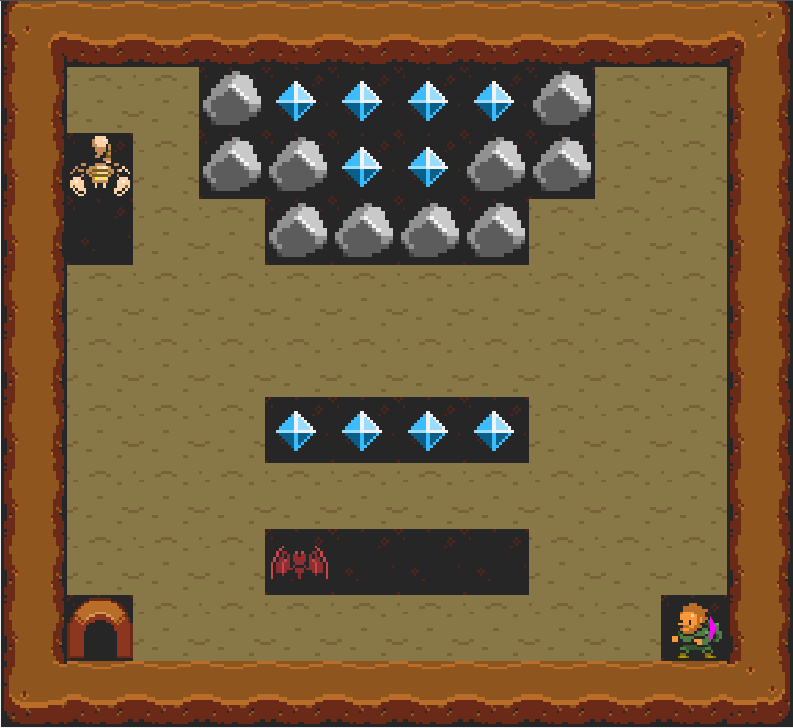
\includegraphics[scale=0.38]{img/CH06/boulderdash.png}
    \caption{Nivel de ejemplo del juego \textit{Boulderdash}.}
    \label{fig:boulderdash-example}
\end{figure}

A continuación se ofrece el contenido de la plantilla que se ha obtenido a la hora de ejecutar
el \textit{script}:

\begin{lstlisting}[language=yaml]
domainFile: domains/boulderdash-domain.pddl
problemFile: problem.pddl
domainName: BoulderDash
cellVariable: null
avatarVariable: null
gameElementsCorrespondence:
  background:
  - null
  wall:
  - null
  sword:
  - null
  dirt:
  - null
  exitdoor:
  - null
  diamond:
  - null
  boulder:
  - null
  avatar:
  - null
  crab:
  - null
  butterfly:
  - null
variablesTypes:
  ?variable: Type
orientationCorrespondence:
  UP: null
  DOWN: null
  LEFT: null
  RIGHT: null
connections:
  UP: null
  DOWN: null
  LEFT: null
  RIGHT: null
actionsCorrespondence:
  TURN-UP: ACTION_UP
  TURN-DOWN: ACTION_DOWN
  TURN-LEFT: ACTION_LEFT
  TURN-RIGHT: ACTION_RIGHT
  MOVE-UP: ACTION_UP
  MOVE-DOWN: ACTION_DOWN
  MOVE-LEFT: ACTION_LEFT
  MOVE-RIGHT: ACTION_RIGHT
  MOVE-UP-GET-GEM: ACTION_UP
  MOVE-DOWN-GET-GEM: ACTION_DOWN
  MOVE-LEFT-GET-GEM: ACTION_LEFT
  MOVE-RIGHT-GET-GEM: ACTION_RIGHT
  DIG-UP: ACTION_UP
  DIG-DOWN: ACTION_DOWN
  DIG-LEFT: ACTION_LEFT
  DIG-RIGHT: ACTION_RIGHT
  EXIT-LEVEL: null
goals:
- goalPredicate: null
  priority: 0
  saveGoal: false
  removeReachedGoalsList:
  - null
\end{lstlisting}

Los campos que aparecen en el fichero son los siguientes:

\begin{enumerate}
    \item \texttt{domainFile}: Nombre del fichero de dominio \texttt{PDDL}. Este campo se genera
    automáticamente a partir de los parámetros utilizados a la hora de ejecutar el \textit{script}.
    
    \item \texttt{problemFile}: Nombre del fichero de problema de salida. Tiene como valor por defecto
    \texttt{problem.pddl}, pero el usuario puede darle el nombre que quiera.
    
    \item \texttt{domainName}: Nombre del dominio. Se genera automáticamente y se obtiene a partir del
    archivo de dominio \texttt{PDDL}.
    
    \item  \label{enum:cell} \texttt{cellVariable}: Variable que se utilizará para representar las celdas. Una
    variable viene precedida por el símbolo ``\texttt{?}'' y se le da el nombre que quiera el usuario. El uso del
    símbolo de interrogación es para que tenga cierta semejanza con la manera en la que se hacen las definiciones
    de variables en \texttt{PDDL}. Por ejemplo, en este caso se ha decidido que dicha variable sea la
    siguiente:
    
    \begin{lstlisting}[language=yaml]
cellVariable: ?c
    \end{lstlisting}
    
    Supongamos que en el dominio \texttt{PDDL} se ha definido el predicado \texttt{(at ?obj - Objeto ?cel - Celda)},
    el cual representa que un determinado objeto \texttt{?obj} se encuentra en una celda \texttt{?cel} determinada.
    En este caso, la variable \texttt{?cel} del predicado se correspondería con la variable que hemos
    definido aquí, la cual es \texttt{?c}. Si este predicado está asociado a algún elemento del juego,
    cuando el traductor se encuentre con dicho elemento sustituirá en este predicado la variable
    \texttt{?c} por su instancia correspondiente, la cual será \texttt{c\_x\_y}, donde \texttt{x}
    es la columna e \texttt{y} la fila donde se encuentra dicho elemento del juego.
    
    \item \texttt{avatarVariable}: Variable que se utilizará para representar al avatar/agente. Por
    ejemplo, en este caso se ha decidido que sea la siguiente:
    
    \begin{lstlisting}[language=yaml]
avatarVariable: ?p
    \end{lstlisting}
    
    Esta variable es especial, ya que cuando se encuentre dicha variable en alguno de los predicados asociados
    al avatar se va a sustituir simplemente por el nombre que le ha dado el usuario. Por ejemplo,
    en este caso se sustituiría por \texttt{p}. Se ha hecho de esta forma debido a que simplifica
    mucho la monitorización del plan, ya que tener una variable que constantemente cambia sus coordenadas
    $x,y$ solo induciría a errores.
    
    \item \texttt{gameElementsCorrespondence}: Este campo sirve para asociar una lista de predicados
    a cada observación (elemento) del juego, de forma que cuando el traductor de estados de observación
    se encuentre con dicha observación, generará los correspondientes predicados instanciando las variables
    de la misma forma que se describió en el punto \ref{enum:cell}, a excepción como se comentó en el
    punto anterior de las variables asociadas al jugador, las cuales se instancian de forma especial.
    Las observaciones se obtienen a partir del fichero que define el juego en formato \texttt{VGDL}, el
    cual recordemos que se pasa como parámetro a la hora de generar la plantilla del archivo de configuración.
    Una observación que aparece siempre es \texttt{background}, la cual representa una celda en la que no
    hay nada. Para este juego en concreto se han definido las siguientes correspondencias:
    
    \begin{lstlisting}[language=yaml]
gameElementsCorrespondence:
  background:
  - (terrain-empty ?c)
  wall:
  - (terrain-wall ?c)
  sword:
  - (terrain-empty ?c)
  dirt:
  - (terrain-ground ?c)
  exitdoor:
  - (at ?e ?c)
  - (terrain-empty ?c)
  diamond:
  - (at ?g ?c)
  - (terrain-empty ?c)
  - (occupied ?c)
  boulder:
  - (at ?boulder ?c)
  - (terrain-empty ?c)
  - (occupied ?c)
  avatar:
  - (at ?p ?c)
  - (terrain-empty ?c)
  crab:
  - (at ?s ?c)
  - (terrain-empty ?c)
  - (occupied ?c)
  butterfly:
  - (at ?b ?c)
  - (terrain-empty ?c)
  - (occupied ?c)    
    \end{lstlisting}
    
    Los predicados que aparecen, como es de suponer, deben ser los que se encuentran en el dominio
    \texttt{PDDL} y deben ser correctos. Otra cosa importante es que se debe mantener un mínimo de consistencia.
    Por ejemplo, si se ha definido que las celdas se representan mediante la variable \texttt{?c}, en
    todos aquellos predicados donde aparezcan celdas debería aparecer dicha variable. En resumen, la nomenclatura
    que se utiliza para definir las variables debe ser consistente, ya que si no se hace de esta forma,
    se pueden llegar a producir errores a la hora de traducir las observaciones del juego.
    
    \item \texttt{variablesTypes}: Este campo representa una correspondencia entre las variables que
    aparecen en los predicados del campo anterior y los tipos de \texttt{PDDL} que el usuario haya definido
    en el dominio. Para este juego en concreto se han definido las siguientes asociaciones:
    
    \begin{lstlisting}[language=yaml]
variablesTypes:
  ?e: Exit
  ?p: Player
  ?boulder: Boulder
  ?g: Gem
  ?b: Bat
  ?s: Scorpion
  ?c: Cell
    \end{lstlisting}
    
    Aunque anteriormente se ha definido cuáles son las variables asociadas a las celdas y al agente,
    sigue siendo necesario especificar su tipo, ya que el usuario podría darle cualquier nombre al
    tipo asociado a dichas variables al no haber un estándar.
    
    \item \texttt{orientationCorrespondence}: Este campo es opcional y solo se utiliza en aquellos
    juegos donde la orientación del personaje sea un factor a tener en cuenta. A cada clave se le
    tiene que asociar el correspondiente predicado que indique que el agente está orientado en esa
    dirección (\texttt{UP} para arriba, \texttt{DOWN} para abajo, \texttt{LEFT} para izquierda
    y \texttt{RIGHT} para derecha). En este caso, los siguientes predicados indican la orientación:
    
    \begin{lstlisting}[language=yaml]
orientationCorrespondence:
  UP: (oriented-up ?p)
  DOWN: (oriented-down ?p)
  LEFT: (oriented-left ?p)
  RIGHT: (oriented-right ?p) 
    \end{lstlisting}
    
    \item \texttt{connections}: Indica la relación de conectividad entre las celdas del juego.
    Esto obliga a que en el dominio se represente el mapa del juego como una cuadrícula. Por tanto, tienen
    que haberse declarado una serie de predicados que indiquen las conexiones entre las celdas. La clave
    \texttt{UP} indica que una celda está encima de la otra, \texttt{DOWN} que una está debajo de la otra,
    \texttt{LEFT} que una está a la izquierda de la otra y \texttt{RIGHT} que una está a la derecha de
    la otra. Un ejemplo de esto se puede ver a continuación:
    
    \begin{lstlisting}[language=yaml]
connections:
  UP: (connected-up ?c ?u)
  DOWN: (connected-down ?c ?d)
  LEFT: (connected-left ?c ?l)
  RIGHT: (connected-right ?c ?r)
    \end{lstlisting}
    
    Es importante destacar que las variables que aparecen en estos predicados no tienen nada que ver
    con las que se han definido en anteriores campos. Cuando se recorra el mapa para generar los relaciones
    de conectividad la variable \texttt{?c} representará la celda actual, la cual está en la posición $(x,y)$.
    La variable \texttt{?u} representará la celda superior a la actual situada en la posición $(x, y-1)$,
    \texttt{?d} la inferior respecto a la actual situada en la posición $(x, y+1)$, \texttt{?l} la izquierda
    respecto a la actual situada en la posición $(x-1, y)$ y \texttt{?r} la derecha respecto a la actual 
    situada en la posición $(x+1, y)$.
    
    \item \texttt{actionsCorrespondence}: Correspondencia entre las acciones definidas en el dominio
    \texttt{PDDL} y las acciones de \texttt{GVGAI}. Las acciones \texttt{PDDL} se obtienen
    a partir del archivo de dominio. Si el nombre de la acción \texttt{PDDL} contiene ciertos
    patrones, se produce una traducción automática a una acción de \texttt{GVGAI}:
    
    \begin{itemize}[label=\textbullet]
        \item Si contiene \textit{up}, la acción se traduciría como \texttt{ACTION\_UP}.
        \item Si contiene \textit{down}, la acción se traduciría como \texttt{ACTION\_DOWN}.
        \item Si contiene \textit{left}, la acción se traduciría como \texttt{ACTION\_LEFT}.
        \item Si contiene \textit{right}, la acción se traduciría como \texttt{ACTION\_RIGHT}.
        \item Si contiene \textit{use}, la acción se traduciría como \texttt{ACTION\_USE}.
        \item Si no contiene ninguno de los patrones anteriores, se traduciría como \texttt{null},
        dejándole al usuario la tarea de asignarle un acción de \texttt{GVGAI}, si es que la hay.
    \end{itemize}
    
    Obviamente, el usuario puede modificar las traducciones a su gusto. Las acciones que tienen
    como traducción \texttt{null} no se tendrán en cuenta a la hora de traducir los planes. También,
    si no se quiere que se tenga en cuenta una acción, bien porque no tenga traducción o bien por otro
    motivo, simplemente bastaría con eliminar dicha acción.
    
    \item \texttt{goals}: Representa la lista de objetivos definida por el usuario. Un objetivo está compuesto
    por un predicado \texttt{PDDL} que representa lo que se quiere alcanzar, la prioridad del objetivo, una
    opción que indica si guardar el objetivo o no una vez que este ha sido alcanzado y un campo opcional
    que contiene una lista de objetivos alcanzados y guardados que deben ser eliminados. Cuanto menor
    sea el valor de la prioridad, más prioridad tendrá dicho objetivo. Puede darse el caso de que haya
    más de un objetivo con la misma prioridad, lo cual implica que no importa el orden en el que se
    completen dichos objetivos. Guardar un objetivo sirve para incluirlo en los próximos estados \texttt{PDDL}
    que genere el traductor de estados de observación, ya que puede ser que al alcanzar dicho objetivo
    se produzca un cambio en el juego que debe ser considerado para alcanzar objetivos posteriores.
    Eliminar un objetivo guardado una vez que se ha alcanzado otro implica que algo que anteriormente
    era verdad ha dejado de serlo, y por tanto, el objetivo a eliminar no será incluido en posteriores
    estados \texttt{PDDL}. Obviamente, para que esto suceda se tiene que haber alcanzado el objetivo a
    eliminar previamente. A continuación se puede ver un ejemplo de esto:
    
    \begin{lstlisting}[language=yaml]
goals:
- goalPredicate: (got g_5_3)
  priority: 1
  saveGoal: no
- goalPredicate: (got g_6_3)
  priority: 1
  saveGoal: no
- goalPredicate: (got g_7_3)
  priority: 1
  saveGoal: no
- goalPredicate: (got g_1_4)
  priority: 1
  saveGoal: no
- goalPredicate: (got g_6_1)
  priority: 1
  saveGoal: no
- goalPredicate: (got g_7_1)
  priority: 1
  saveGoal: no
- goalPredicate: (got g_7_9)
  priority: 1
  saveGoal: no
- goalPredicate: (got g_9_10)
  priority: 1
  saveGoal: no
- goalPredicate: (exited-level)
  priority: 2
  saveGoal: no
- goalPredicate: (got g_16_9)
  priority: 1
  saveGoal: no
    \end{lstlisting}
    
    Aquí se indica que el agente primero debe recoger 9 gemas en cualquier orden (debido a que tienen la misma
    prioridad) y que, una vez que las ha obtenido, debe salir del nivel. Ninguno de estos objetivos tiene que ser
    guardado, y ninguno tiene una lista de objetivos a eliminar una vez que se haya alcanzado. Es importante destacar
    que, a la hora de indicar los objetivos, las variables de los predicados se sustituyen por objetos (instancias
    concretas de las variables). Por ejemplo, si nos fijamos en el primer objetivo, vemos que el predicado con la
    variable instanciada es \texttt{(got g\_5\_3)} (hay una gema en la posición $x = 5, y= 7$ ), mientras que el
    predicado como tal sería \texttt{(got ?g)}. Por tanto, es necesario conocer cómo se instancian las variables,
    así como también la posición de los elementos en el mapa.
\end{enumerate}

%%%%%%%%%%%%%%%%%%%%%%%%%%%%%%%%%%%%%%%%%%%%%%%%%%%%%%%%%%%%%%%%%%%%%%%%%%%%%%%%
%                    Capitulo 7: Diseño software del sistema                   %
%%%%%%%%%%%%%%%%%%%%%%%%%%%%%%%%%%%%%%%%%%%%%%%%%%%%%%%%%%%%%%%%%%%%%%%%%%%%%%%%

\chapter{Diseño software del sistema}

\section{Implementación}

Comentar brevemente la implementación llevada a cabo.

\section{Arquitectura software del sistema}

Comentar la arquitectura software del sistema.

\begin{figure}[H]
    \centering
    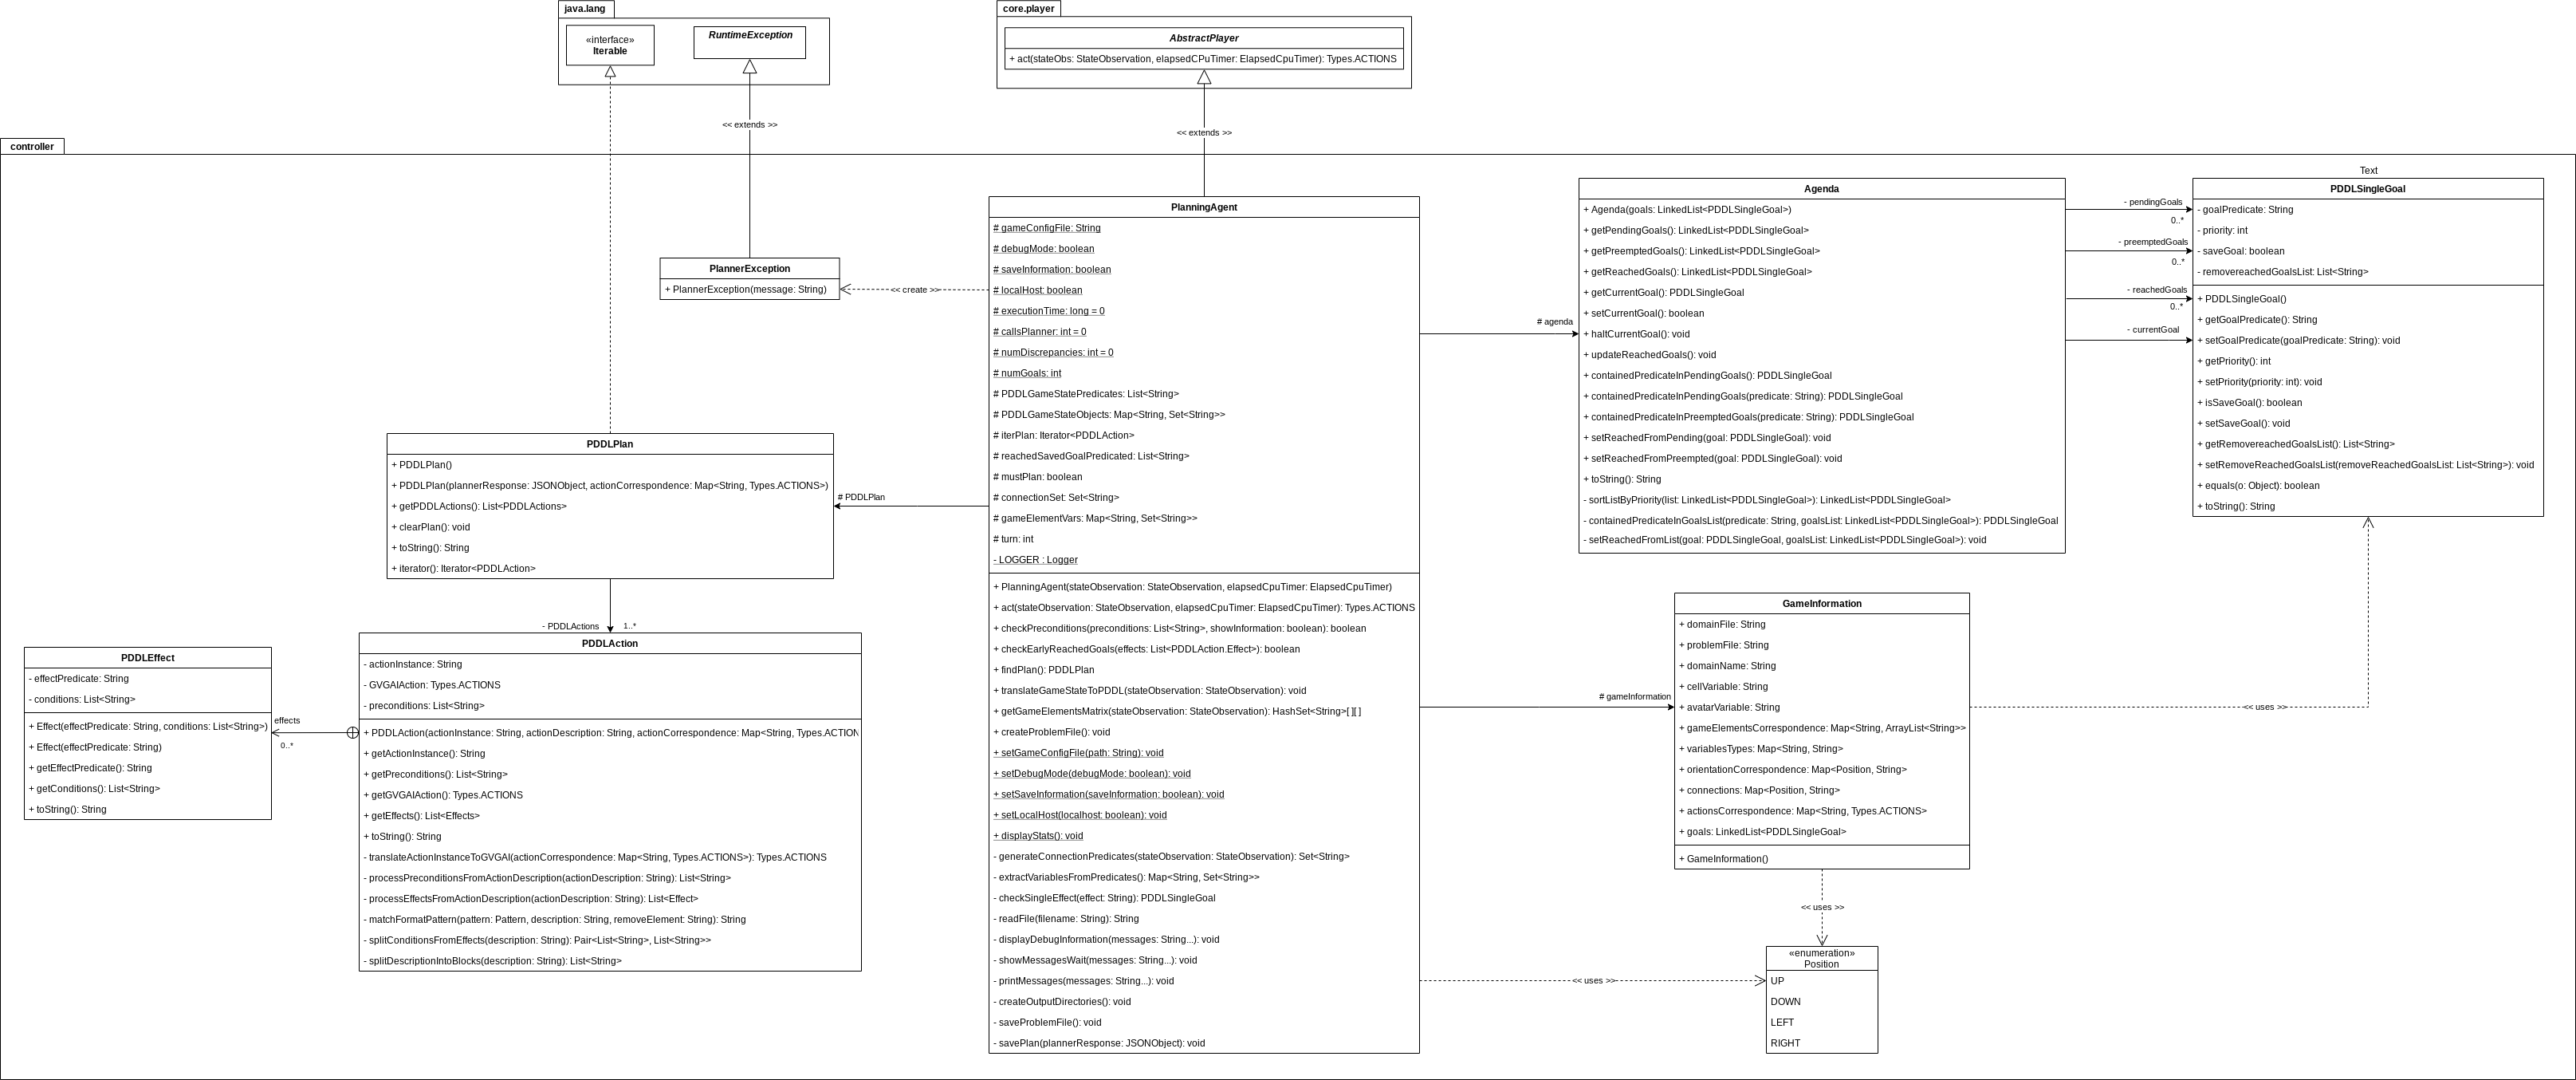
\includegraphics[angle=90, origin=c, scale=0.18]{img/CH07/class_diagram.png}
    \caption{Diagrama de clases.}
    \label{fig:class_diagram}
\end{figure}

\begin{figure}[H]
    \centering
    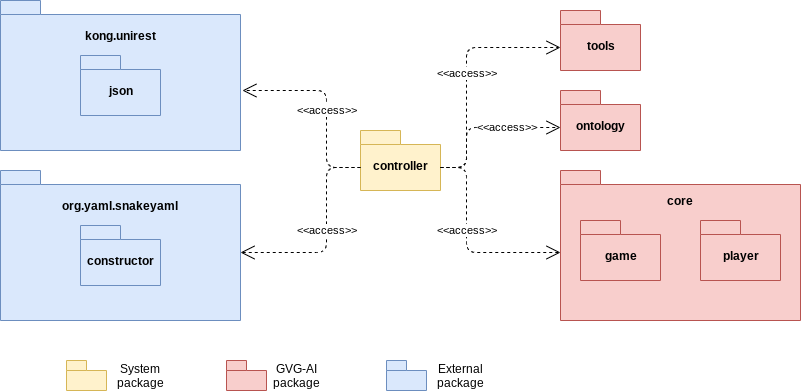
\includegraphics[scale=0.48]{img/CH07/package_diagram.png}
    \caption{Diagrama de paquetes.}
    \label{fig:package_diagram}
\end{figure}

\section{Descripción de las clases}

\begin{figure}[H]
    \centering
    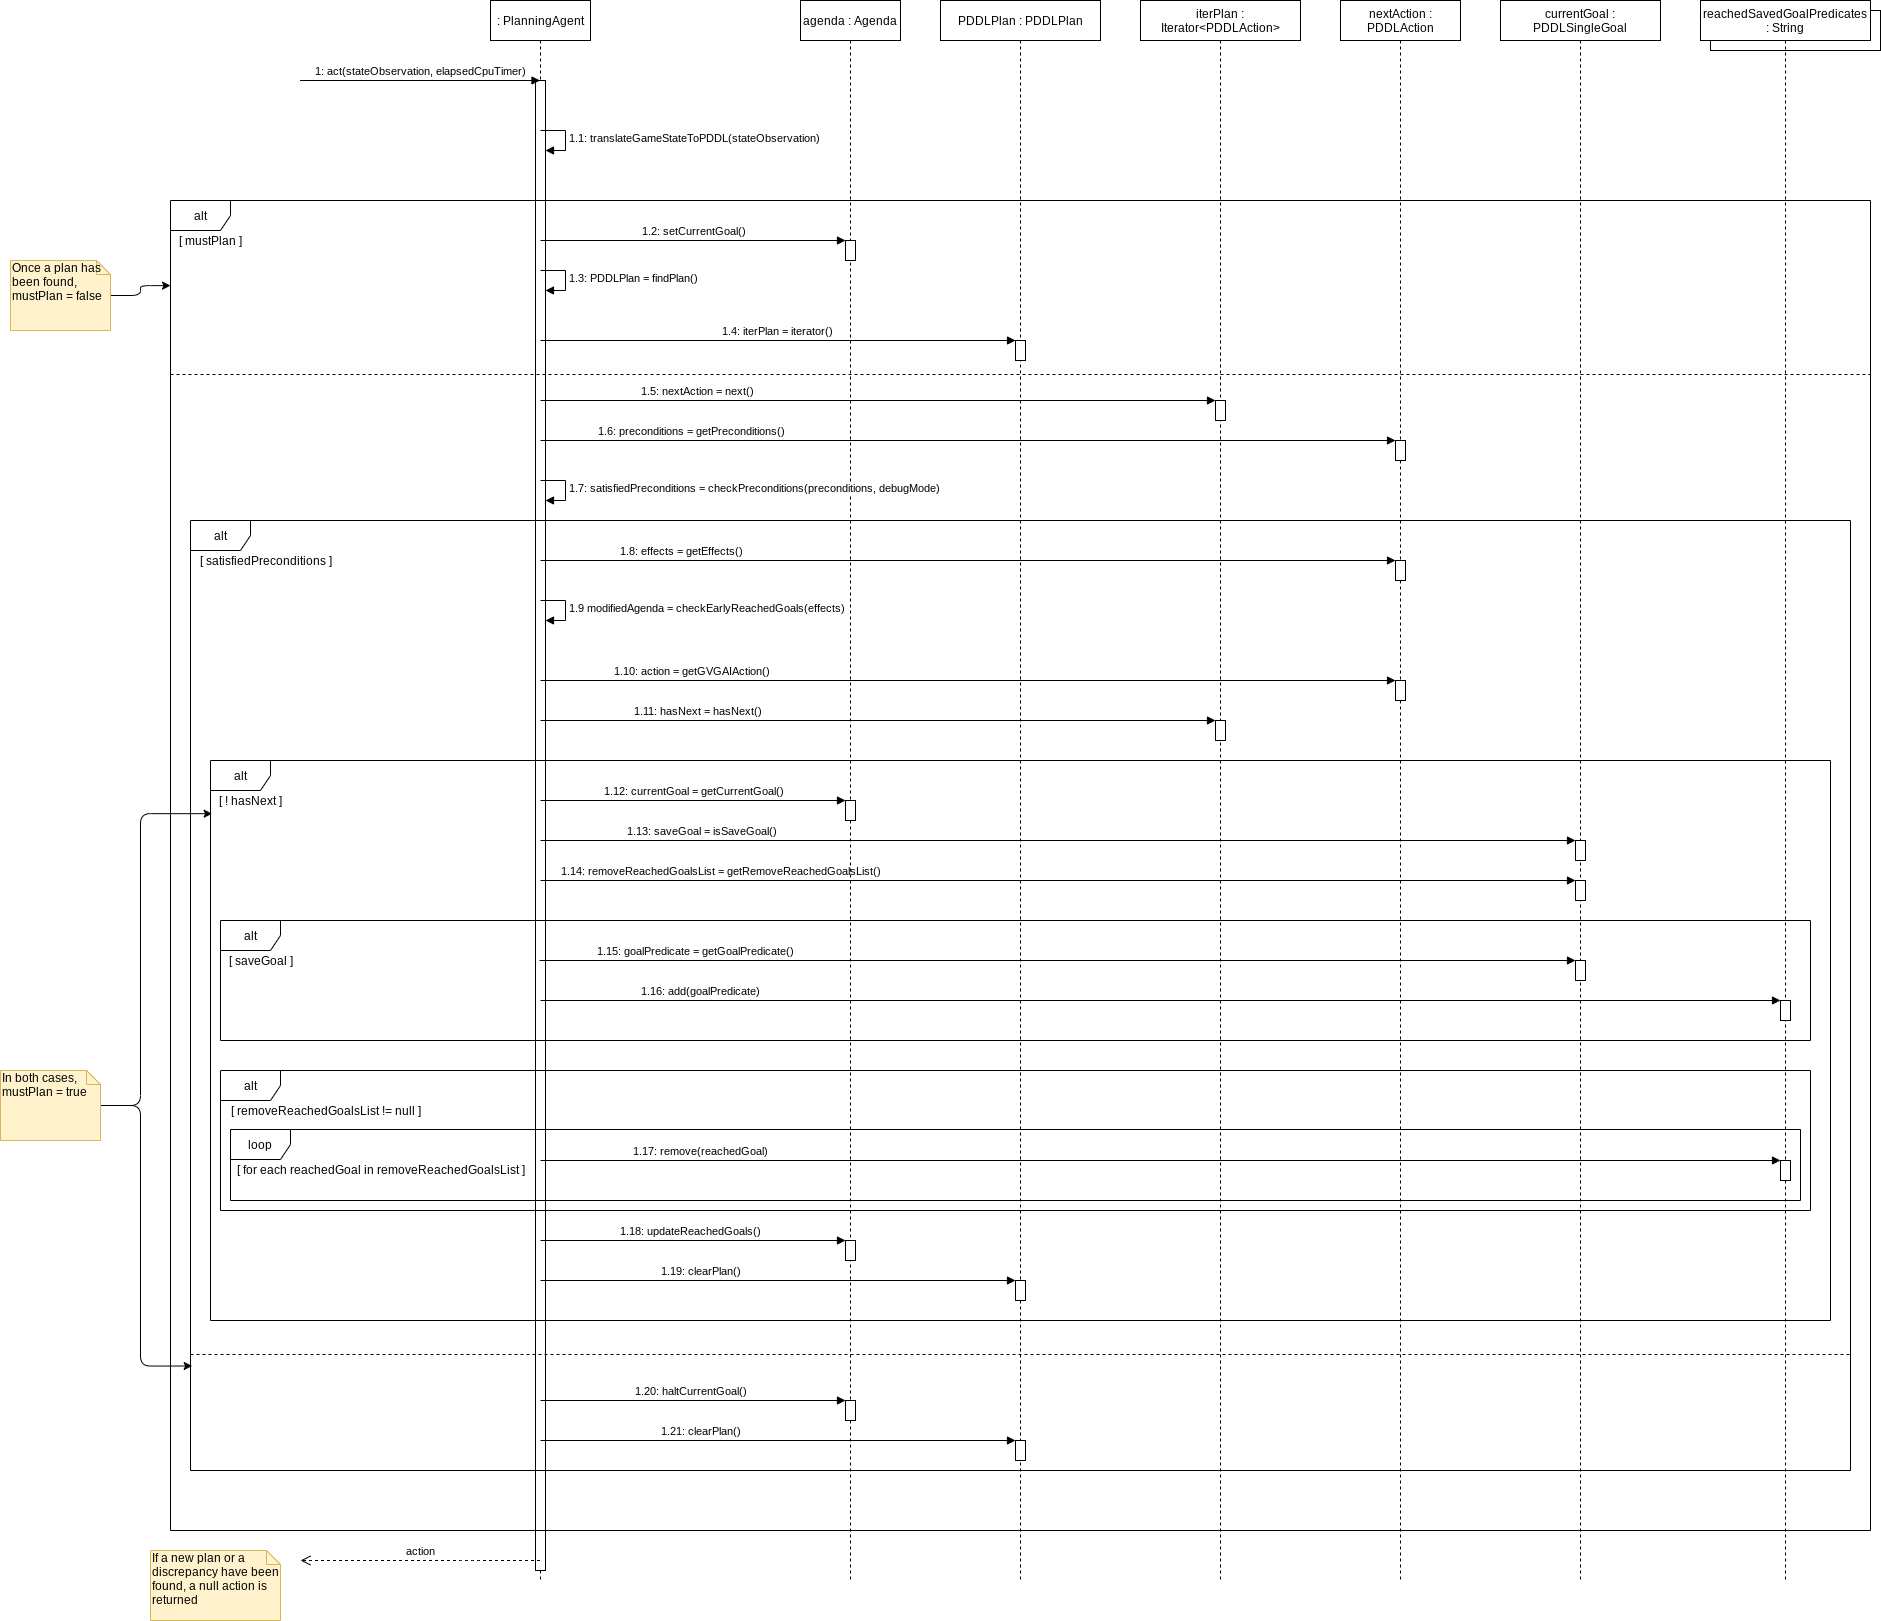
\includegraphics[scale=0.22]{img/CH07/sequence_diagram.png}
    \caption{Diagrama de secuencia del método \texttt{act()}.}
    \label{fig:sequence_diagram}
\end{figure}

%%%%%%%%%%%%%%%%%%%%%%%%%%%%%%%%%%%%%%%%%%%%%%%%%%%%%%%%%%%%%%%%%%%%%%%%%%%%%%%%
%                    Capitulo 8: Experimentacion                               %
%%%%%%%%%%%%%%%%%%%%%%%%%%%%%%%%%%%%%%%%%%%%%%%%%%%%%%%%%%%%%%%%%%%%%%%%%%%%%%%%

\chapter{Experimentación}

Una vez que el sistema ha sido implementado y validado, es necesario realizar un estudio
de su funcionamiento. Este estudio consiste en llevar a cabo una serie de experimentos,
los cuales pretenden poner a prueba dos aspectos fundamentales del sistema:

\begin{enumerate}
    \item La capacidad que tiene para generar problemas \texttt{PDDL} de forma
    automática a partir de los estados del juego.
    \item La capacidad que tiene para responder a los cambios dinámicos que
    se producen en los juegos.
\end{enumerate}

Para llevar a cabo estos experimentos se han escogido los siguientes juegos:

% Comentar aquí los juegos, relacionandolos con las imagenes
\begin{itemize}[label=\textbullet]
    \item \textbf{\textit{Boulderdash}}. El objetivo del juego consiste en recoger 9 de
    las gemas que hay esparcidas a lo largo de todo el mapa y llegar a la salida
    sin morir en el intento (ver figura \ref{fig:boulderdash}). En el mapa hay también
    esparcidos dos tipos de enemigos: las mariposas y los cangrejos, los cuales matarán al agente
    si chocan con él. Si dos enemigos chocan entre sí, se generará una gema nueva. En el
    juego original, las rocas son afectadas por la gravedad, de manera que si la casilla debajo de una
    de ellas está excavada (es decir, es una casilla vacía), la roca caerá hasta toparse
    con una casilla que contenga tierra, un muro, una gema u otra roca. Una roca cayendo puede matar
    al agente si colisiona con este. Sin embargo, debido a la extrema dificultad que supone
    simular este sistema de físicas en un dominio \texttt{PDDL}, se trabaja con una versión
    simplificada del juego donde las rocas no caen y pueden ser excavadas utilizando el pico
    del que dispone el agente, de forma que estas rocas desaparecen del mapa.
    
    Esta versión del juego, a pesar de ser simplificada, es no determinista, ya que el
    comportamiento de los enemigos es totalmente aleatorio. Este no determinismo introduce
    por tanto cierto dinamismo en el juego, ya que los enemigos pueden interponerse en el
    camino del agente y matarlo. Es aquí donde el monitor va a jugar un papel clave,
    ya que gracias a él se podrá determinar si algún enemigo se interpone entre el agente
    y el objetivo al que se dirige.
    
    \item \textbf{\textit{Ice and Fire}}. En este juego, el agente tiene que atravesar una especie
    de laberinto hasta la salida, el cual está lleno de obstáculos como pinchos, fuego y hielo
    (ver figura \ref{fig:ice_and_fire}). Estos obstáculos matarán al jugador si entra en contacto
    directo con ellos. Sin embargo, las casillas que contienen fuego pueden ser atravesadas si el
    agente dispone de unas botas de fuego. Análogamente, se pueden atravesar las casillas que
    contienen hielo si se tienen las botas de hielo. Se pueden llevar equipados los dos tipos
    de botas simultáneamente, de forma que se pueden atravesar ambos tipos de obstáculos. Los
    pinchos, por desgracia, no pueden atravesarse. A lo largo del mapa hay también una serie
    de monedas que pueden ser recogidas para aumentar la puntuación del jugador, aunque esto es más
    bien secundario. Este juego es totalmente determinista ya que, al no haber enemigos u otros
    personajes en el mapa, no se pueden llegar a producir eventos exógenos que obliguen a modificar
    un plan obtenido.
    
    \item \textbf{\textit{Labyrinth Dual}}. Aquí el agente también tiene que atravesar un laberinto
    hasta la salida esquivando los pinchos y atravesando una serie de casillas para las que requiere
    un traje en específico de los que se pueden encontrar por el mapa (ver figura \ref{fig:labyrinth_dual}).
    El traje rojo permite atravesar los muros de color gris oscuro y el traje azul permite atravesar
    las muros de color azul. El agente solo puede llevar equipado un traje a la vez. Si ya tiene equipado
    uno y coge el otro, se cambia de traje, perdiendo la capacidad de atravesar las casillas que
    antes podía. Por tanto, hay que tener cierto cuidado a la hora de coger un traje, ya que
    en algunas ocasiones cambiar de traje puede llegar a encerrar al agente, impidiéndole llegar
    a la meta. A pesar de eso, el juego es totalmente determinista, ya que no hay factores
    externos que puedan impedir que un plan hasta un objetivo determinado sea llevado a cabo.
\end{itemize}

\begin{figure}[H]
    \centering
    \begin{subfigure}[t]{.5\textwidth}
        \centering
        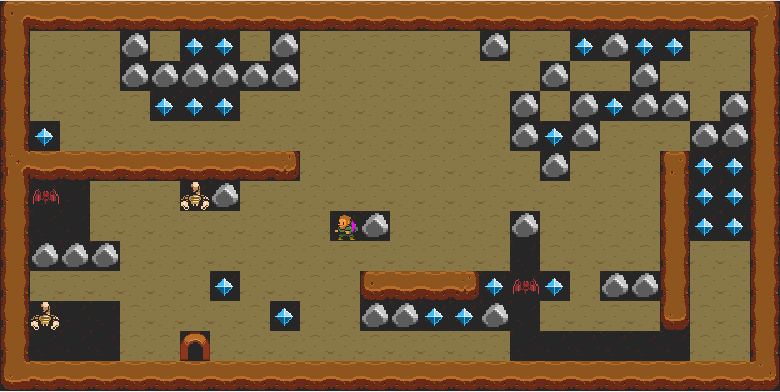
\includegraphics[scale=0.3]{img/CH08/boulderdash.png}
        \caption{\textit{Boulderdash}.}
        \label{fig:boulderdash}
    \end{subfigure}%
    \begin{subfigure}[t]{.5\textwidth}
        \centering
        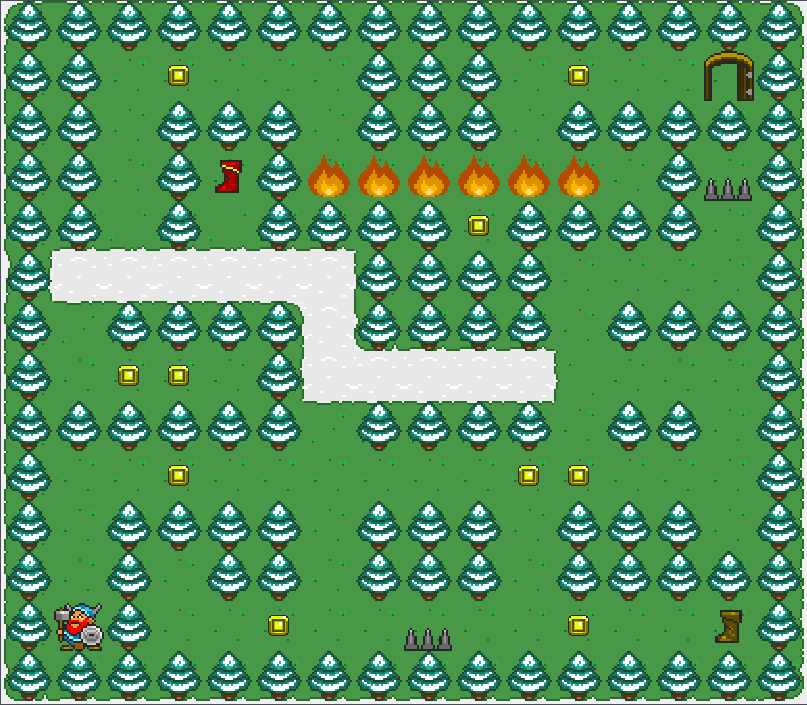
\includegraphics[scale=0.25]{img/CH08/ice_and_fire.png}
        \caption{\textit{Ice and Fire}.}
        \label{fig:ice_and_fire}
    \end{subfigure}
    \par\bigskip
    \begin{subfigure}[t]{0.5\textwidth}
        \centering
        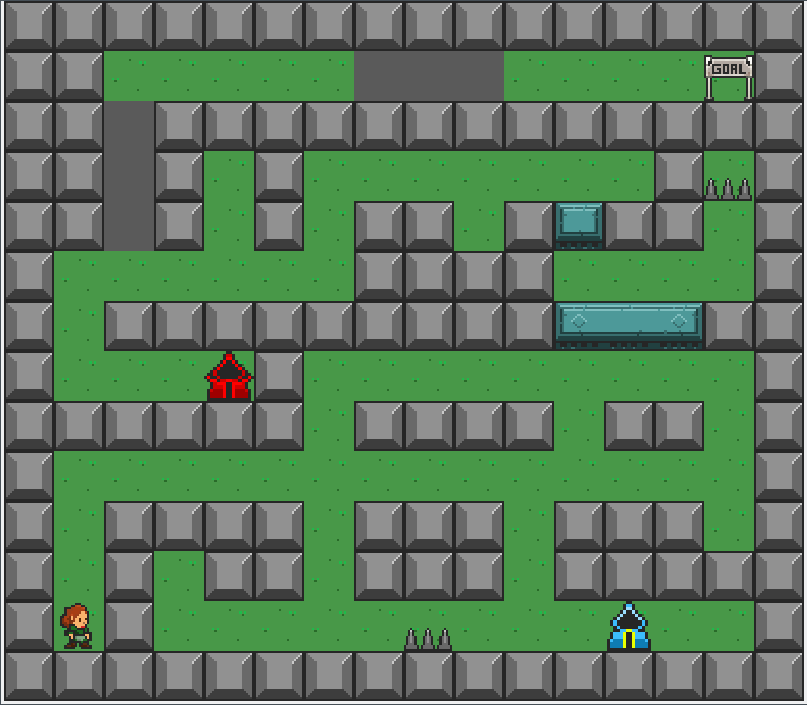
\includegraphics[scale=0.25]{img/CH08/labyrinth_dual.png}
        \caption{\textit{Labyrinth Dual}.}
        \label{fig:labyrinth_dual}
    \end{subfigure}
    \caption{Juegos con los que se han realizado los experimentos.}
    \label{fig:games}
\end{figure}

Para cada juego se ha creado su dominio \texttt{PDDL}, intentando hacer una representación lo más
fiel posible del juego. En la tabla \ref{tab:info-domains} puede el número de predicados, de tipos y
de acciones que conforman cada uno de los dominios. Adicionalmente, debido a que la planificación es
un proceso lento, es importante destacar que a la hora de construir el sistema se han modificado tanto el
tiempo máximo que tiene el agente para dar una respuesta, el cual ha pasado a ser 40 segundos (originalmente 40
milisegundos), como el tiempo máximo que se espera antes de descalificar al agente, el cual es ahora
500 segundos (anteriormente 50 milisegundos).

\begin{table}[H]
\centering
\begin{tabular}{|c|ccc|}
\hline
\textbf{Juego} & \textbf{Predicados} & \textbf{Tipos} & \textbf{Acciones} \\ \hline
\textit{Boulderdash} & 15 & 9 & 17 \\ \hline
\textit{Ice and Fire} & 13 & 10 & 14 \\ \hline
\textit{Labyrinth Dual} & 12 & 9 & 14 \\ \hline
\end{tabular}
\caption{Información sobre los dominios creados para cada juego.}
\label{tab:info-domains}
\end{table}

\section{Generación de problemas}

Para comprobar la generación de problemas se han hecho pruebas con cada uno de los cinco
niveles de los tres juegos anteriormente mencionados. Para cada nivel de cada juego se ha
creado un archivo de configuración en el cual se ha especificado la información correspondiente,
además de decir los objetivos concretos que se deben alcanzar en cada nivel. En cada ejecución se
ha obtenido información del número de predicados y objetos que que conforman el estado inicial
del primer archivo de problema generado\footnote{En general, va a haber muy poca variabilidad entre
dichos números para archivos de problema posteriores, y como en algunos juegos hay más
elementos al principio del juego, esto nos da una idea de cuánto se tarda en generar el problema más
grande.}, el tiempo total de ejecución desde que empieza el juego, el tiempo de generación
de los predicados de conectividad entre casillas, el tiempo medio de traducción de
un estado de observación, el tiempo medio de generación un archivo de problema
y la suma de los tres tiempos anteriores, lo cual nos da una idea de cuánto se tarda en
generar un problema completo de media. Se han realizado 3 ejecuciones de cada nivel, de modo
que los resultados obtenidos para los tiempos son una media de esas tres ejecuciones.

En la tabla \ref{tab:exp-results} se pueden ver los resultados obtenidos. Como puede observarse,
en todos los casos se generan problemas con más de 1000 predicados y cerca de 350-400 objetos.
Puede verse también que el tiempo medio total para generar un problema es del orden de centésimas
de segundo. Generar problemas de este tamaño a mano podría llevar días e incluso semanas, además de
que se pueden cometer errores a la hora de crearlos, lo cual puede retrasar dicha creación aún
más tiempo. Por tanto, hacer uso de esta arquitectura permite ahorrar muchísimo tiempo de trabajo
y permite detectar de forma más rápida los posibles errores que puedan aparecer a la hora de crear
un archivo de problema.

Si observamos los tiempos individuales que suman dicho tiempo total de generación de problema, se
puede ver que las fases de traducción del estado de observación y la generación del archivo
de problema tienen un tiempo medio del orden de milésimas de segundo, mientras que el proceso
que más tarda es la generación de los predicados de conectividad, el cual tarda un tiempo medio
del orden de las centésimas de segundo. Esto es normal, ya que los predicados de conectividad representan
una gran parte de los predicados del problema. Para un mapa dado de tamaño $w \times h$, siendo $w$
la anchura y $h$ la altura, el número de predicados de conectividad, $PC$, viene dado por la expresión
\eqref{eq:pc}:

\begin{equation}
    PC = 4 \cdot 2 \; pred + 2 ((w-2) + (h-2)) \cdot 3 \; pred + (w-2)(h-2) \cdot 4 \; pred
    \label{eq:pc}
\end{equation}

\begin{landscape}
\begin{table}[]
\centering
\resizebox{1.51\textwidth}{!}{%
\begin{tabular}{|c|c|cccccccc|}
\hline
\textbf{Juego} &
  \textbf{Nivel} &
  \textbf{Objetivos} &
  \textbf{\begin{tabular}[c]{@{}c@{}}Predicados problema\\ inicial\end{tabular}} &
  \textbf{\begin{tabular}[c]{@{}c@{}}Objetos problema\\ inicial\end{tabular}} &
  \textbf{\begin{tabular}[c]{@{}c@{}}Tiempo medio\\ ejecución (s)\end{tabular}} &
  \textbf{\begin{tabular}[c]{@{}c@{}}Tiempo medio\\ generación predicados\\ conectividad (s)\end{tabular}} &
  \textbf{\begin{tabular}[c]{@{}c@{}}Tiempo medio\\ traducción estado\\ de observación (s)\end{tabular}} &
  \textbf{\begin{tabular}[c]{@{}c@{}}Tiempo medio\\ generación archivo\\ de problema (s)\end{tabular}} &
  \textbf{\begin{tabular}[c]{@{}c@{}}Tiempo medio total\\ generación problema\\ (s)\end{tabular}} \\ \hline
\multirow{5}{*}{\textit{Boulderdash}}    & \textbf{0} & 10 & 1735 & 400 & 0.4967 & 0.0313 & 0.0024 & 0.0038 & 0.0375 \\ \cline{2-10} 
                                         & \textbf{1} & 10 & 1721 & 393 & 0.428  & 0.0323 & 0.0029 & 0.0039 & 0.0392 \\ \cline{2-10} 
                                         & \textbf{2} & 10 & 1717 & 391 & 0.5293 & 0.0347 & 0.0034 & 0.0044 & 0.0425 \\ \cline{2-10} 
                                         & \textbf{3} & 10 & 1733 & 399 & 0.7487 & 0.0327 & 0.0049 & 0.0048 & 0.0423 \\ \cline{2-10} 
                                         & \textbf{4} & 10 & 1731 & 398 & 0.4403 & 0.0317 & 0.0030 & 0.0039 & 0.0386 \\ \hline
\multirow{5}{*}{\textit{Ice and Fire}}   & \textbf{0} & 3  & 1215 & 391 & 0.417  & 0.027  & 0.0026 & 0.003  & 0.0326 \\ \cline{2-10} 
                                         & \textbf{1} & 3  & 1234 & 410 & 0.4827 & 0.0307 & 0.0028 & 0.0056 & 0.0390 \\ \cline{2-10} 
                                         & \textbf{2} & 3  & 1235 & 411 & 0.522  & 0.0273 & 0.0031 & 0.0045 & 0.0349 \\ \cline{2-10} 
                                         & \textbf{3} & 3  & 1219 & 395 & 0.4587 & 0.0323 & 0.0029 & 0.0061 & 0.0413 \\ \cline{2-10} 
                                         & \textbf{4} & 3  & 1210 & 386 & 0.697  & 0.0273 & 0.0031 & 0.0055 & 0.0359 \\ \hline
\multirow{5}{*}{\textit{Labyrinth Dual}} & \textbf{0} & 3  & 1085 & 369 & 0.4503 & 0.0303 & 0.0029 & 0.0043 & 0.0376 \\ \cline{2-10} 
                                         & \textbf{1} & 2  & 1069 & 380 & 0.3847 & 0.0303 & 0.0027 & 0.0045 & 0.0376 \\ \cline{2-10} 
                                         & \textbf{2} & 3  & 1073 & 378 & 0.4107 & 0.0287 & 0.0024 & 0.0029 & 0,0339 \\ \cline{2-10} 
                                         & \textbf{3} & 3  & 1083 & 376 & 0.41   & 0.0297 & 0.0031 & 0.0052 & 0.038  \\ \cline{2-10} 
                                         & \textbf{4} & 2  & 1079 & 363 & 0.5623 & 0.029  & 0.0029 & 0.0062 & 0.0381 \\ \hline
\end{tabular}%
}
\caption{Resultados de la experimentación.}
\label{tab:exp-results}
\end{table}
\end{landscape}

\section{Respuesta a cambios dinámicos}

Para facilitar el estudio de la respuesta que ofrece el sistema a los cambios dinámicos en
los juegos, se ha creado un nuevo nivel del juego \textit{Boulderdash}, que es el
único de la lista que contiene no determinismo al tener enemigos que se mueven por el mapa
aleatoriamente, y se ha fijado una semilla aleatoria, de forma que el comportamiento de los enemigos
fuese el deseado. El nuevo nivel puede observarse en la figura \ref{fig:discrepancy_1}. Se ha creado
también un archivo de configuración en el cual se han especificado qué gemas tiene que coger
el agente antes de salir del nivel. La primera de ellas es la gema que está justo encima suyo,
la cual está rodeada de enemigos.

Después de obtener un plan hasta dicha gema, comienza la ejecución de éste. Mientas el agente
intenta avanzar, una mariposa se le cruza en el camino, tal y como puede verse en la figura
\ref{fig:discrepancy_2}. El monitor, al hacer un estudio de las precondiciones de la siguiente
acción a ejecutar, detecta una discrepancia, ya que la celda justo arriba del agente está
ocupada por un enemigo, algo que no se esperaba. Es entonces cuando se le indica al gestor
de objetivos que se ha producido una discrepancia y que se debe seleccionar un nuevo objetivo,
que resulta ser la gema que se encontraba a la izquierda de la posición inicial del agente.

Se obtiene un plan hasta dicha gema y, tal y como se puede ver en la figura \ref{fig:discrepancy_3},
el agente alcanza el nuevo objetivo propuesto. Vemos por tanto que el agente ha conseguido
responder a la aparición de un enemigo en su camino, algo que no estaba previsto cuando obtuvo
el plan, deteniendo por tanto la ejecución del plan actual y cambiando a un nuevo objetivo.

\begin{figure}[H]
    \centering
    \begin{subfigure}[t]{0.32\textwidth}
        \centering
        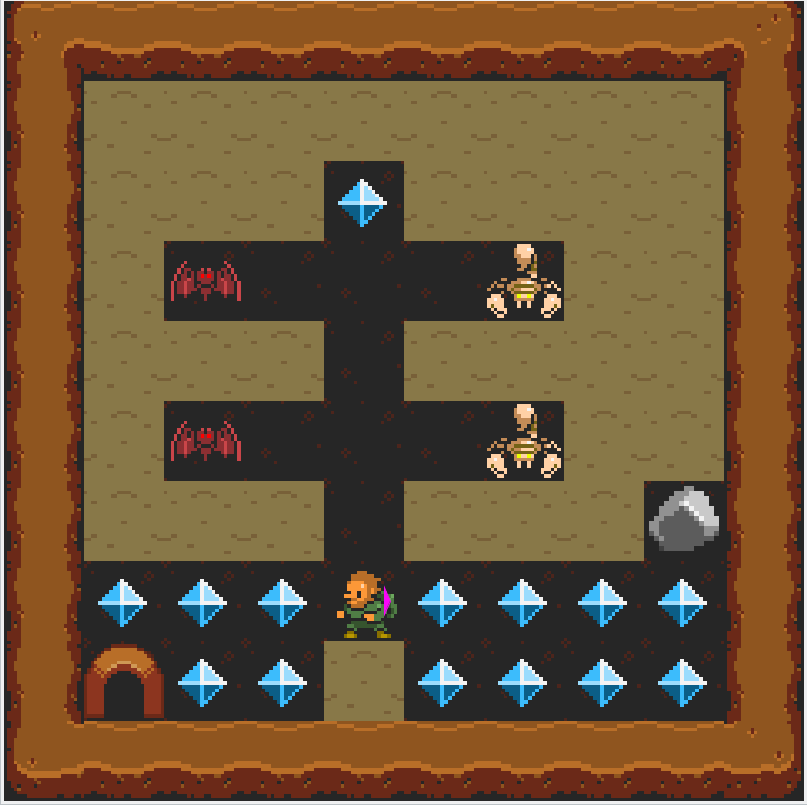
\includegraphics[scale=0.2]{img/CH08/discrepancy_1.png}
        \caption{Estado inicial del juego.}
        \label{fig:discrepancy_1}
    \end{subfigure}%
    \begin{subfigure}[t]{0.32\textwidth}
        \centering
        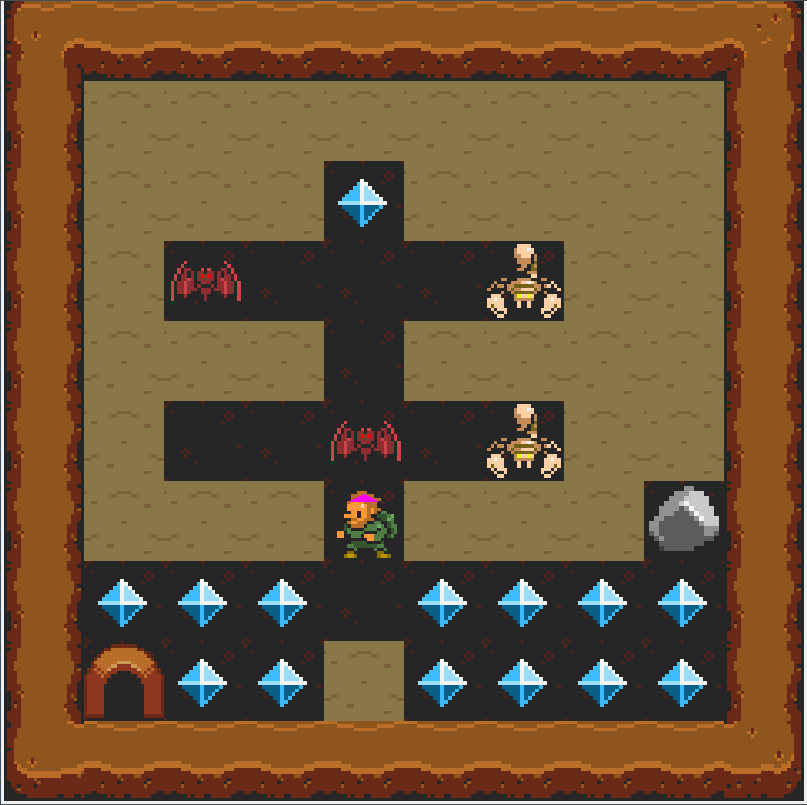
\includegraphics[scale=0.2]{img/CH08/discrepancy_2.png}
        \caption{Mariposa bloquea el camino.}
        \label{fig:discrepancy_2}
    \end{subfigure}%
    \begin{subfigure}[t]{0.32\textwidth}
        \centering
        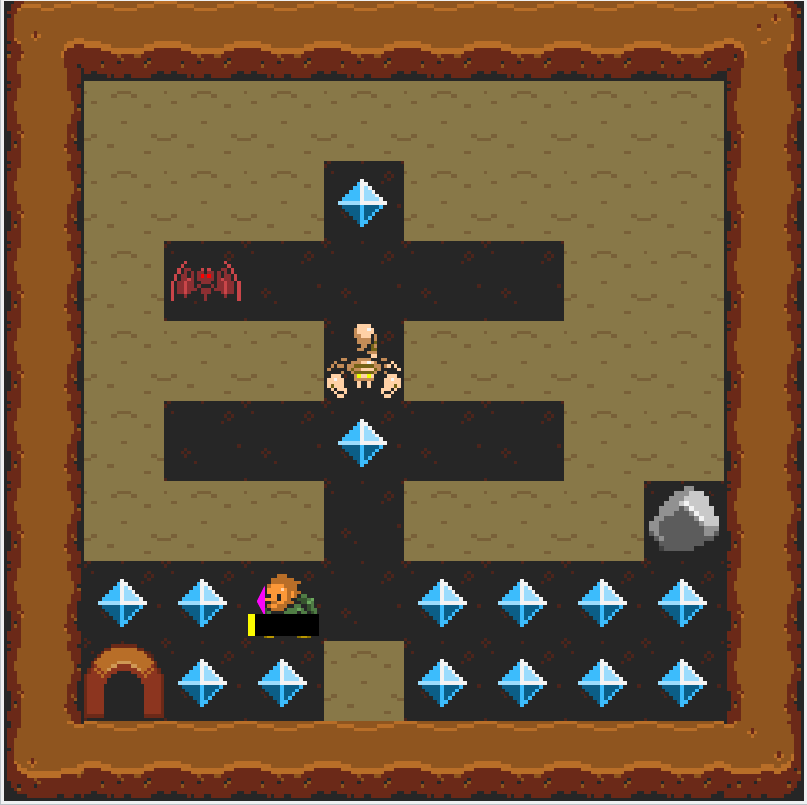
\includegraphics[scale=0.2]{img/CH08/discrepancy_3.png}
        \caption{Agente cambia de objetivo y lo alcanza.}
        \label{fig:discrepancy_3}
    \end{subfigure}
    \caption{Ejemplo de respuesta a cambios dinámicos en el entorno en \textit{Boulderdash}.}
    \label{fig:discrepancies}
\end{figure}

%%%%%%%%%%%%%%%%%%%%%%%%%%%%%%%%%%%%%%%%%%%%%%%%%%%%%%%%%%%%%%%%%%%%%%%%%%%%%%%%
%                       Capitulo 9: Conclusiones                               %
%%%%%%%%%%%%%%%%%%%%%%%%%%%%%%%%%%%%%%%%%%%%%%%%%%%%%%%%%%%%%%%%%%%%%%%%%%%%%%%%

\chapter{Conclusiones}


\section{Trabajos futuros}

\newpage

% Incluir la bibliografia completa
\nocite{*}
\printbibliography[heading=bibintoc]

\end{document}

